\section{Dienste}
\begin{frame}{}
    \begin{center}
        Dienste im Netz
     \end{center}
\end{frame}

\begin{frame}{Monitoring}
    \only<1-2>{
        \begin{center}
            \vspace{-0.1\textheight}
            \noindent\fbox{\noindent
                \only<1>{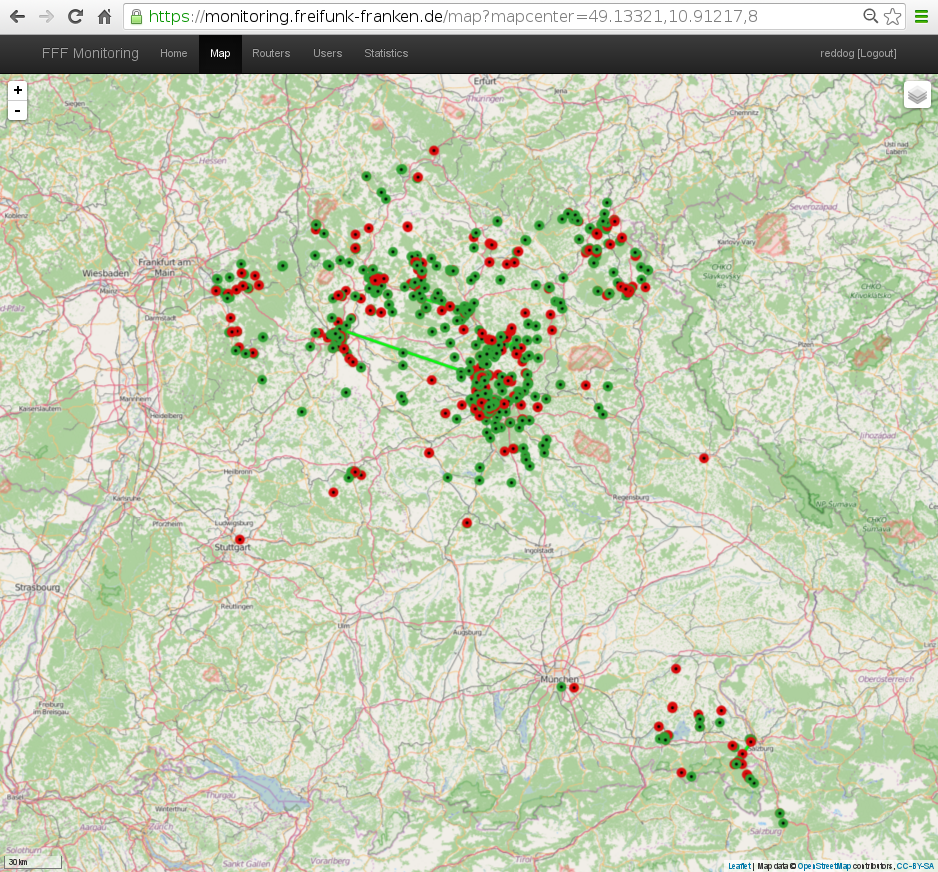
\includegraphics[width=0.77\dimexpr\textwidth-2\fboxsep-2\fboxrule\relax]{img/monitoring-map.png}}%
                \only<2>{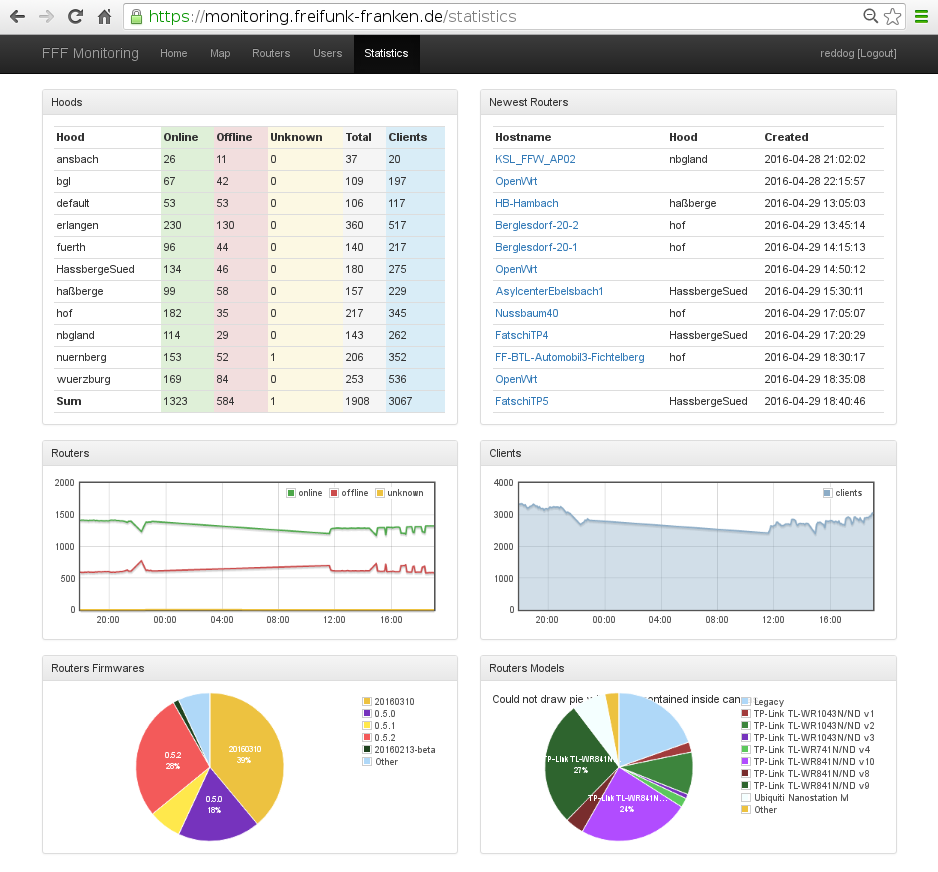
\includegraphics[width=0.77\dimexpr\textwidth-2\fboxsep-2\fboxrule\relax]{img/monitoring-statistic.png}}%
            }
            \vspace{-0.1\textheight}
        \end{center}
    }
    \only<3-4>{
        \begin{itemize}
            \item Alfred
            \begin{itemize}
                \item XML
                \item alle 5 Minuten
                \item Multicast
            \end{itemize}
            \item Alfred-Proxy
            \begin{itemize}
                \item Multicast Daten werden gelesen
                \item An das Monitoring geschickt
            \end{itemize}
            \item Alfred-Legacy Provider
            \begin{itemize}
                \item Kann die Daten wir Netmon laden
            \end{itemize}
        \item<4> {\color{red}Problem!} Beides nur auf dem Netmon-Server
        \end{itemize}
    }
\end{frame}

\begin{frame}{Domain-Name-System}
    \begin{itemize}
        \item fff.community
        \begin{itemize}
            \item Langer Name, aber
            \item Keine Kollision
        \end{itemize}
        \item Mehrere DNS Server
        \item Zonen-Synchronisation über dig axfr
        \item Subdelegation an synchronisierte Hosts möglich
        \item Automatisierte reverse delegation
    \end{itemize}
\end{frame}

\begin{frame}{Firmware Bau}
    \begin{itemize}
        \item Basiert auf OpenWrt
        \item ,,Eigenes'' Framework (Buildscript)
        \item Zentrales ,,files'' Verzeichnis
        \begin{itemize}
            \item<2> {\color{red}Problem!} Keine Abhängigkeiten; Schlecht zu pflegen
        \end{itemize}
        \item Board-Support-Packages
        \begin{itemize}
            \item Ein .config
            \item Überschreibende ,,files''
        \end{itemize}
        \item Template System für versch. Communities
        \item Versionierung: YYYYmmDD
    \end{itemize}
\end{frame}
